\chapter{More}

%%%%%%%%%%%%%%%%%%%%%%%%%%%%%%%%%%%%%%%%%%%%%%%%%%%%%%%%%%%%%%%%%%%%%%%%%%%%%%%%
\section{References and links}
\label{sec:references}

We use the \verb|hyperref| package to produce a pdf with hyperlinks. We also use the \verb|cleveref| package for facilitating references. Using the \verb|\cref| command will automatically use the correct prefix. You can also refer to multiple things at once by using multiple arguments, or you can refer to a range using \verb|\crefrange|. For more information, see the documentation\footnote{\url{http://mirrors.ctan.org/macros/latex/contrib/cleveref/cleveref.pdf}}.

References can be cited with the \verb|\cite| command, which produces something like \cite{lessard16,lessard2015optimal,sundararajan2020analysis,tmm}. The \verb|cite| package ensures the citations are ordered nicely and compressed when possible.


%%%%%%%%%%%%%%%%%%%%%%%%%%%%%%%%%%%%%%%%%%%%%%%%%%%%%%%%%%%%%%%%%%%%%%%%%%%%%%%%
\section{Figures and tables}

\paragraph{Figures}

We use the standard \verb|figure| environment for figures. Diagrams should be placed in separate files in the \texttt{graphics/} folder and should use the \texttt{standalone} package. You can then use \verb|includegraphics| as in \Cref{fig:sample} to include the figure in your document. If you are using \verb|pdflatex|, you can also use \verb|includegraphics| to include PDF, JPEG, PNG, or other formats, but not EPS.

\begin{figure}[htb]
	\centering
	\begin{tabular}{cc}
		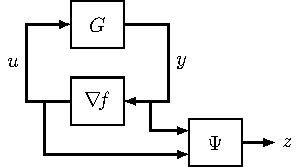
\includegraphics{text_figure} & 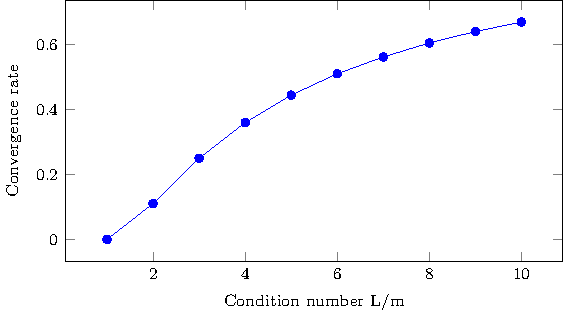
\includegraphics{test_plot}
	\end{tabular}
	\caption{Figure captions should be long and descriptive because people actually read them, unlike the rest of the text. (Left) A block diagram make using Tikz. (Right) A plot made using Pgfplots. Note that the figures are not scaled, so the text size in the figures is consistent with the rest of the document. The source files for the figures are in the \texttt{graphics/} folder.}
  \label{fig:sample}
\end{figure}

\paragraph{Tables}

The \verb|booktabs| package, which includes commands such as \verb|\toprule|, \verb|\midrule|, and \verb|\bottomrule|, can be used to make nice tables. In general, never use vertical lines to separate columns. For more style tips on how to make nice tables, see\footnote{\url{https://people.inf.ethz.ch/markusp/teaching/guides/guide-tables.pdf}}. Here is an example of a nice table\footnote{\url{https://lazyscientist.wordpress.com/2021/07/23/make-better-tables-in-latex-using-booktabs/}}.

\begin{table}[htbp]
	\centering
	\caption{Gravimetric analysis of silver halides in a 1.27-mL sample of sea water.}
	  \begin{tabular}{lSSSSS}
		  \toprule
		  \multicolumn{1}{c}{} & \multicolumn{4}{c}{Test Tubes} & \multicolumn{1}{c}{} \\
		  \cmidrule(rl){2-5} 
			Qty of Sample                & {A}           & {B}           & {C}           & {D}    & {Avg}             \\
		  \cmidrule(r){1-1} \cmidrule(rl){2-5} \cmidrule(l){6-6}
			Mass (g)                     & 1.399         & 1.32          & 1.328         & 1.408  & 1.364           \\
			Density (g/mL)               & 1.10          & 1.04          & 1.05          & 1.109  & 1.07            \\
			Mass w/ Precipitate (g)      & 13.443        & 13.401        & 13.348        & {---}  & 13.397          \\
			Mass AgCl (\num{e-2} g)      & 9.0           & 9.2           & 8.7           & {---}  & 8.9             \\
			Moles AgCl (\num{e-4} mol)   & 6.28          & 6.42          & 6.08          & {---}  & 6.50            \\
		  \bottomrule
	  \end{tabular}
	\label{tab:grav4}
\end{table}